\documentclass{article}

\usepackage{times}
\usepackage{amsmath, amssymb}
\usepackage{bm}
\usepackage{upgreek}

\usepackage{graphicx}
\usepackage{float}
\usepackage{subfigure}

\title{\Large Integrated System Biology Report}
\author{Department of Systems Science \\ Ma Zhenjia, ID: 6930-29-4499 \\ 
	Instructing Teacher: Ishii Shin}
\date{2017/08/18}

\begin{document}
	\maketitle
	
	\section{Problem Description}
		Train an agent that automatically search the solution path in a maze
		using \textit{TD0} algorithm.
			
	\section{Major Algorithm}
		The \textit{TD0} method of reinforcement learning is based on a sampling method
		that takes sample movement in the given state space to collect samples, and 
		improve the value function according to the observed reward.
		The notation \textit{TD} refers to the full name \textit{Temporary Difference} that
		use a difference between the current value and the temporary value to 
		update the value function, which is
		\[
			V(x, y) \leftarrow V(x, y) + \alpha(\sum_{t=0}^Tr_t\gamma^t+\gamma^{T+1}V(x', y')
				- V(x, y))
		\]
		where $\sum_{t=0}^Tr_t\gamma^t+\gamma^{T+1}V(x_t, y_t)$ refers to the temporary
		value for $T+1$ step and $\alpha$ refers to the training rate.
		\textit{TD0} refers to the algorithm when $T=0$ and thus
		\[
			V(x, y) \leftarrow V(x, y) + \alpha(r+\gamma V(x', y')
				- V(x, y))
		\]
		Take sufficient large quantity of samples and updates the value function following the 
		formula above until convergent. The discount parameter $\gamma$ is set to be $0.95$.
	
	\section{Program Implementation}
		The coding is constructed by the following parts.
		\subsection{Environment: \textit{Maze\_ENV.py}}
			Environment class that describe the property and the action of the environment (maze),
			which is totally determined by the problem definition.
			It contains the query of the current state, the current reward, whether it is a terminate
			state or not, and the receptor of the action taken followed by the process
			of state dynamic and returning whether or not it is a legal action.
		\subsection{Agent: \textit{Maze\_AGNT.py}}
			Agent functions that interacts with the environment object.
			The function \textit{ExecEpi()} refers to the process to take a complete
			episode until terminate while \textit{TD0()} is a sub-function that returns
			the \textit{TD0}-evaluated \textit{$\epsilon$ - greedy} driven action selection result,
			where $\epsilon$ is a hyper-parameter controls the trade-off between
			the exploration and the exploitation in sampling search.
		\subsection{Trainer: \textit{Maze\_Train.py}}
			Trainer that find the optimal value function for this problem.
			Call the \textit{Agent} to run for $10000$ times and promise the convergence
			of value function.
	
	\section{Variated Studying Rate}
		There are two parameters, searching trade-off $\epsilon$ and the training rate $\alpha$,
		that are vital to the proper convergence of the algorithm, especially $\epsilon$.
		At the early stage of iteration, the value for most of the states are $0$, which refers that
		their value have not been updated yet. Thus in these area, the \textit{TD0} value can make
		little difference and the program is supposed to search more explorative, which require
		$\epsilon$ to be as large as possible to improve the chance for variance states to be reached.
		However, at the later stage, where according to the \textit{TD0} update, 
		we have already get a rough sketch of the hole state space. At this time, the value function
		we got plays a more important part when making decision. The algorithm is supposed to
		take action that is more likely to lead to the goal, and that require
		$\epsilon$ to be as small as possible, which stands in contrast with the constrain in early
		stage. To tackle this problem, in this report, a variated parameter is used that
		\[
			\epsilon_t = \epsilon_0c^{f(t)}
		\]
		where $c$ is discount constant in $(0, 1)$ and $f(t)$ is a monotonous function of times step
		$t$. So this method promise the algorithm to do more exploration at the beginning,
		and turn to focus on exploiting the likely states later on.
		
		The training rate $\alpha$ also takes the similar idea, that at the beginning, we want
		a high training rate to make the value function quickly get close to the true value,
		and as the iteration goes on, this rate is supposed to be as small as possible
		to make smooth approach to the true value and prevent a large variance.
		
	\section{Result}
		The convergence result of value function is shown below
		\begin{figure}[ht]
			\center
			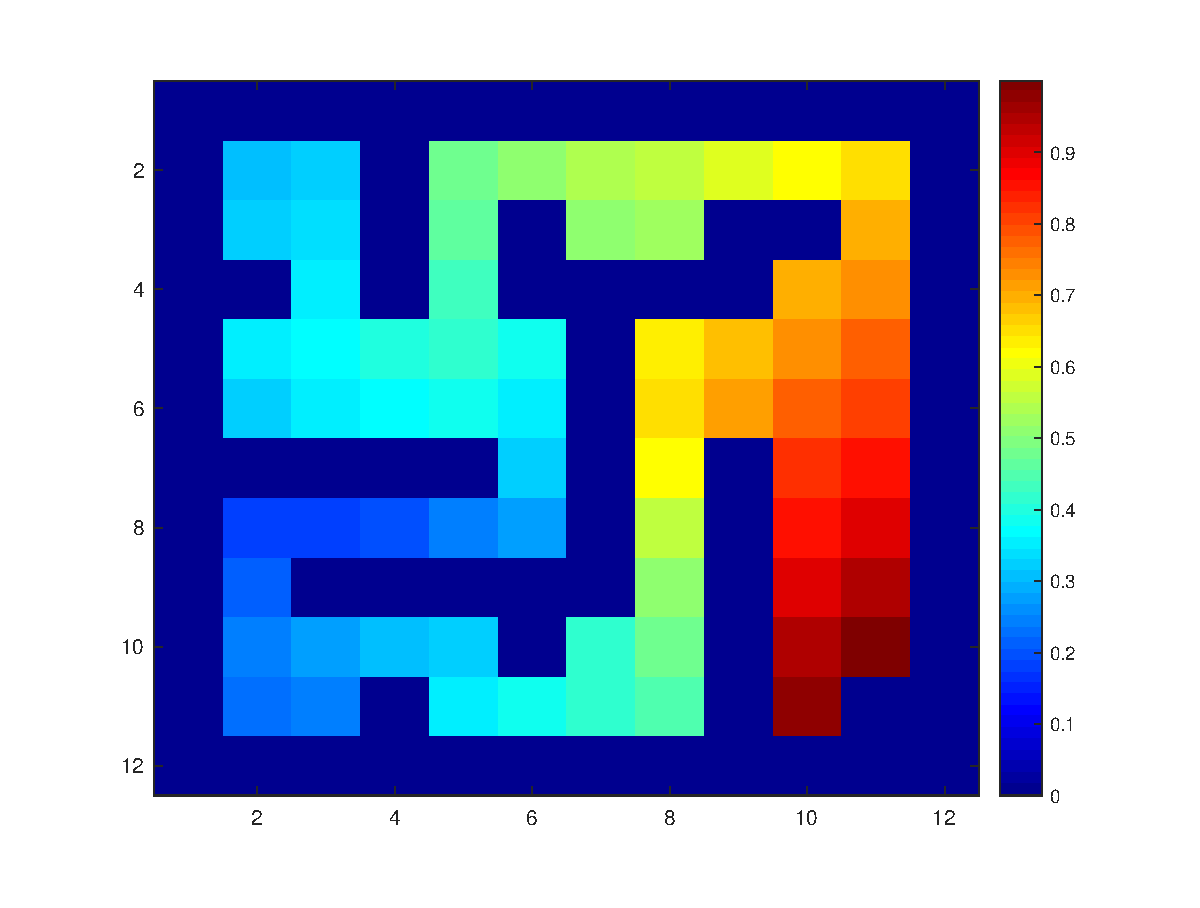
\includegraphics[width=0.8\textwidth]{/Users/admin/Documents/GitHub/Maze/Fig2.eps}
			\caption{Value Function}
		\end{figure}
		The value for start point is arount $3.072$, which that according to the definition of 
		value function and reward, the convergence value for a certain state should be 
		\[
			V(s) = \gamma^{d(s, g)}
		\]
		where $d(s, g)$ denotes the distant from $s$ to goal. So the required steps from 
		start point to the goal could be calculated by
		\[
			d(s, g) = \frac{\ln V(s)}{\ln \gamma} \approx 23
		\]
		which meets the human result for the maze problem.
		
		The training curve for it is shown below
		\begin{figure}[ht]
			\center
			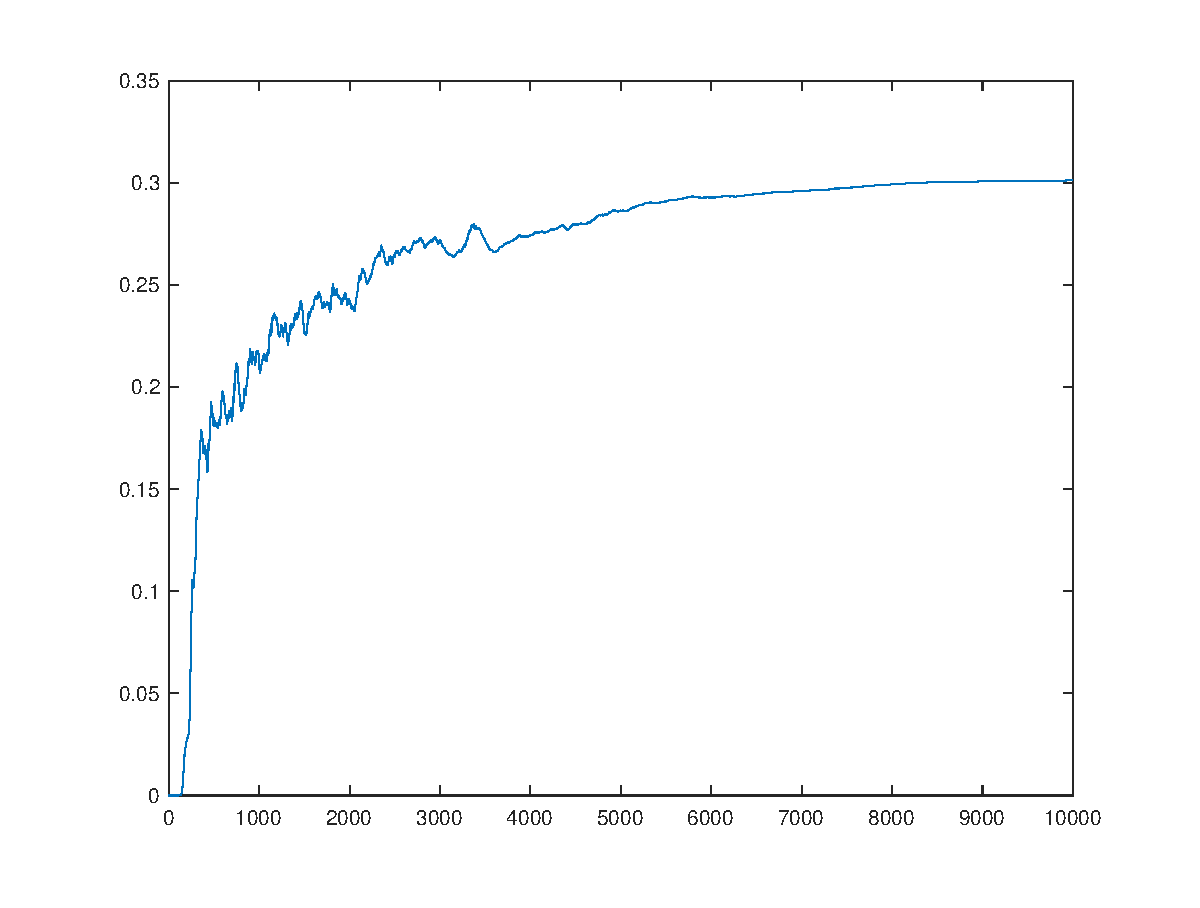
\includegraphics[width=0.8\textwidth]{/Users/admin/Documents/GitHub/Maze/Fig1.eps}
			\caption{Training Curve with discount rate 0.95}
			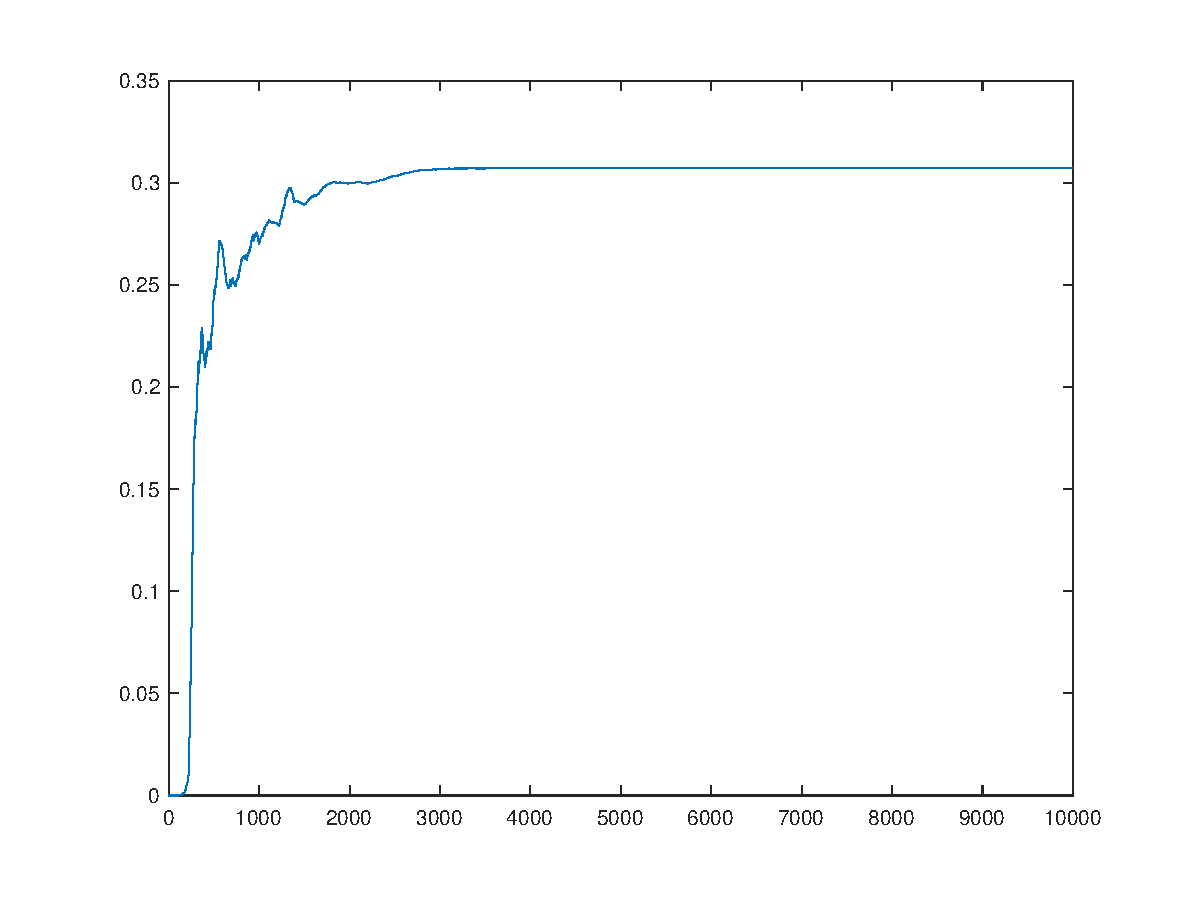
\includegraphics[width=0.8\textwidth]{/Users/admin/Documents/GitHub/Maze/Fig3.eps}
			\caption{Training Curve with discount rate 0.8}
		\end{figure}
		
		As shown in the figure, the curve started to converge after a quite long period since
		the discount rate is set to be large. If the discount rate is set to be smaller.
		the training curve would become
		which makes a quick convergence to the true value.
		However, effectiveness of algorithm in this report is promised by the selection of
		a sufficient long period for almost free search at the early stage, controlled by 
		the discount process been executed every 200 complete episode.
		If the discount rate is set to be too low and there is no minimum undiscounted 
		episode constrain, the algorithm may converge to a local maximum or even
		may not be able to get a solution.
		
		The implement source code is uploaded on 
		\textit{https://github.com/mazhenjia007/Maze}
	\section{Reference}
		Sutton, Richard S., and Andrew G. Barto. Reinforcement learning: An introduction. Vol. 1. No. 1. Cambridge: MIT press, 1998.
\end{document}